\documentclass[11pt,letterpaper]{article}

% ── Packages ──────────────────────────────────────────────────
\usepackage[margin=1in]{geometry}
\usepackage{titlesec}
\usepackage{enumitem}
\usepackage{booktabs}
\usepackage{tabularx}
\usepackage{graphicx}
\usepackage{xcolor}
\usepackage{hyperref}
\usepackage{fancyhdr}
\usepackage{amsmath}
\usepackage{tcolorbox}
\usepackage{multicol}
\usepackage{caption}
\usepackage{tikz}
\usetikzlibrary{shapes.geometric, arrows.meta, positioning, fit, calc}

% ── Colors ────────────────────────────────────────────────────
\definecolor{stevens}{RGB}{163,31,52}       % Primary/Brand Red
\definecolor{darkgray}{RGB}{60,60,60}
\definecolor{lightgray}{RGB}{240,240,240}
\definecolor{accentblue}{RGB}{30,80,140}

% ── Hyperref Setup ────────────────────────────────────────────
\hypersetup{
	colorlinks=true,
	linkcolor=stevens,
	urlcolor=accentblue,
	citecolor=darkgray,
	plainpages=false
}

% ── Header / Footer ──────────────────────────────────────────
\pagestyle{fancy}
\fancyhf{}
\fancyhead[L]{\small\textcolor{darkgray}{Institution or Organization Name}}
\fancyhead[R]{\small\textcolor{darkgray}{Semester or Term}}
\fancyfoot[C]{\thepage}
\renewcommand{\headrulewidth}{0.4pt}

% ── Section Formatting ───────────────────────────────────────
\titleformat{\section}
{\Large\bfseries\color{stevens}}{\thesection}{1em}{}[\vspace{-0.5em}\rule{\textwidth}{0.4pt}]
\titleformat{\subsection}
{\large\bfseries\color{darkgray}}{\thesubsection}{1em}{}

% ── tcolorbox Styles ─────────────────────────────────────────
\tcbset{
	objective/.style={colback=lightgray, colframe=stevens, 
		fonttitle=\bfseries, title=#1, boxrule=0.5pt, arc=2pt},
	infobox/.style={colback=blue!5, colframe=accentblue, 
		fonttitle=\bfseries, title=#1, boxrule=0.5pt, arc=2pt},
	deliverable/.style={colback=green!5, colframe=green!40!black,
		fonttitle=\bfseries, title=#1, boxrule=0.5pt, arc=2pt},
	warning/.style={colback=red!5, colframe=stevens,
		fonttitle=\bfseries, title=#1, boxrule=0.5pt, arc=2pt}
}

% ══════════════════════════════════════════════════════════════
\begin{document}
	
	% ── Title Page ───────────────────────────────────────────────
	\pagenumbering{Alph}
	\begin{titlepage}
		\centering
		\vspace*{2cm}
		
		{\Huge\bfseries\color{stevens} Lesson Plan: Module Name\par}
		\vspace{0.5cm}
		{\LARGE\color{darkgray} Module Subtitle or Primary Topics\par}
		
		\vspace{1.5cm}
		\rule{0.6\textwidth}{1pt}
		\vspace{1.5cm}
		
		{\Large\textbf{Course or Project Title}\par}
		
		\vspace{1.5cm}
		
		\begin{tabular}{rl}
			\textbf{Student/Author:}  & Name \\
			\textbf{Project Advisor:} & Instructor/Advisor Name \\
			\textbf{Program:}         & Degree/Program Name \\
			\textbf{Institution:}     & Institution Name \\
			\textbf{Date Range:}      & Start Date -- End Date \\
		\end{tabular}
		
		\vspace{2cm}
		
		\begin{tcolorbox}[colback=lightgray, colframe=darkgray, width=0.85\textwidth, arc=2pt]
			\centering\small
			Insert a brief abstract or summary of this lesson plan. Describe the scope, the core activities, and the ultimate goal of the module.
		\end{tcolorbox}
		
		\vfill
		{\small\textcolor{darkgray}{Email Address}}
	\end{titlepage}
	
	% ── Table of Contents ────────────────────────────────────────
	\pagenumbering{roman}
	\tableofcontents
	\newpage
	\pagenumbering{arabic}
	
	% ══════════════════════════════════════════════════════════════
	\section{Module Overview}
	% ══════════════════════════════════════════════════════════════
	
	\begin{tcolorbox}[objective={Module Learning Objectives}]
		Upon completion of this module, the student will be able to:
		\begin{enumerate}[label=\textbf{LO-\arabic*}]
			\item Insert Learning Objective 1
			\item Insert Learning Objective 2
			\item Insert Learning Objective 3
		\end{enumerate}
	\end{tcolorbox}
	
	\subsection{Context Within the Project}
	
	Describe how this module fits into the broader timeline or curriculum. What came before this, and what will build upon it?
	
	\subsection{Prerequisites}
	
	Students beginning this module should have:
	\begin{itemize}[leftmargin=2em]
		\item Prerequisite Skill or Knowledge 1
		\item Prerequisite Skill or Knowledge 2
		\item Required Hardware or Software Configuration
	\end{itemize}
	
	\newpage
	% ══════════════════════════════════════════════════════════════
	\section{Session Schedule}
	% ══════════════════════════════════════════════════════════════

	Provide a brief introduction to the schedule.

	\begin{table}[ht!]
		\centering
		\caption{Module session breakdown.}
		\label{tab:schedule}
		\renewcommand{\arraystretch}{1.4}
		\begin{tabularx}{\textwidth}{c l X}
			\toprule
			\textbf{Session} & \textbf{Focus Area} & \textbf{Key Activities} \\
			\midrule
			N+1 & Topic 1 & Detailed description of activities for the first session. \\
			N+2 & Topic 2 & Detailed description of activities for the second session. \\
			N+3 & Topic 3 & Detailed description of activities for the third session. \\
			N+4 & Topic 4 & Detailed description of activities for the fourth session. \\
			\bottomrule
		\end{tabularx}
	\end{table}

	\newpage
	% ══════════════════════════════════════════════════════════════
	\section{Session N+1: Session Topic}
	\label{sec:session1}
	% ══════════════════════════════════════════════════════════════
	
	\subsection{Objectives}
	
	\begin{itemize}[leftmargin=2em]
		\item Specific goal 1
		\item Specific goal 2
	\end{itemize}
	
	\subsection{Topic Section}
	
	Body text explaining the topic, theoretical background, or instructions.
	
	% Example Equation
	\begin{equation}
		y = mx + b
		\label{eq:example}
	\end{equation}
	
	% Example Warning Box
	\begin{tcolorbox}[warning={Common Pitfalls}]
		\begin{itemize}
			\item \textbf{Pitfall 1:} Explanation and how to avoid it.
			\item \textbf{Pitfall 2:} Explanation and how to avoid it.
		\end{itemize}
	\end{tcolorbox}
	
	% Example Infobox / Exercise
	\begin{tcolorbox}[infobox={Exercise: Exercise Name}]
		Instructions for a specific exercise or thought experiment for the student.
	\end{tcolorbox}
	
	% Example Deliverable Box
	\begin{tcolorbox}[deliverable={Session N+1 Deliverable}]
		\textbf{Deliverable Name} --- Description of what needs to be turned in, the format, and specific requirements.
	\end{tcolorbox}
	
	\newpage
	% ══════════════════════════════════════════════════════════════
	\section{Session N+2: Session Topic}
	\label{sec:session2}
	% ══════════════════════════════════════════════════════════════
	
	% Example TikZ Architecture Diagram (Empty Skeleton)
	\begin{figure}[ht!]
		\centering
		\resizebox{0.85\textwidth}{!}{%
			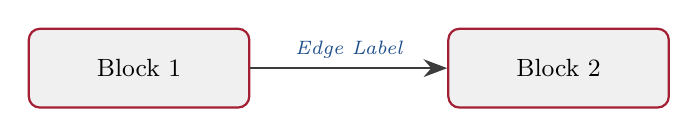
\begin{tikzpicture}[
				node distance=2cm and 2.5cm,
				state/.style={rectangle, draw=stevens, fill=lightgray, thick, rounded corners,
					minimum width=2.8cm, minimum height=1cm, align=center, font=\small},
				arrow/.style={-{Stealth[length=3mm]}, thick, color=darkgray},
				elabel/.style={font=\scriptsize\itshape, color=accentblue}
				]
				
				% Nodes
				\node[state] (node1) {Block 1};
				\node[state, right=of node1] (node2) {Block 2};
				
				% Arrows
				\draw[arrow] (node1) -- (node2) node[midway, above, elabel] {Edge Label};
				
			\end{tikzpicture}%
		}
		\caption{Describe what this diagram illustrates.}
		\label{fig:example_diagram}
	\end{figure}
	
	Additional sections for sessions N+3, N+4, etc. can be copied from the structure above.
	
	\newpage
	% ══════════════════════════════════════════════════════════════
	\section{Hardware / Software Reference}
	\label{sec:resources}
	% ══════════════════════════════════════════════════════════════
	
	\begin{table}[ht!]
		\centering
		\caption{Required components or software tools.}
		\label{tab:hardware}
		\renewcommand{\arraystretch}{1.3}
		\begin{tabularx}{\textwidth}{l l X}
			\toprule
			\textbf{Item} & \textbf{Qty} & \textbf{Purpose} \\
			\midrule
			Tool or Component 1 & X & Reason it is needed \\
			Tool or Component 2 & Y & Reason it is needed \\
			\bottomrule
		\end{tabularx}
	\end{table}
	
	% ══════════════════════════════════════════════════════════════
	\section{Assessment Rubric}
	% ══════════════════════════════════════════════════════════════
	
	\begin{table}[ht!]
		\centering
		\caption{Module assessment rubric.}
		\label{tab:rubric}
		\renewcommand{\arraystretch}{1.3}
		\begin{tabularx}{\textwidth}{X c c}
			\toprule
			\textbf{Assessment Item} & \textbf{Weight} & \textbf{Due} \\
			\midrule
			Deliverable 1 & XX\% & Date or Session \\
			Deliverable 2 & XX\% & Date or Session \\
			\bottomrule
		\end{tabularx}
	\end{table}
	
	\newpage
	% ══════════════════════════════════════════════════════════════
	\section{Recommended Resources}
	% ══════════════════════════════════════════════════════════════
	
	\subsection{Documentation}
	\begin{enumerate}[leftmargin=2em]
		\item Author or Org, ``Title,'' Year.
	\end{enumerate}
	
	\subsection{Textbooks}
	\begin{enumerate}[leftmargin=2em]
		\item Author, \textit{Title}, Publisher, Year.
	\end{enumerate}
	
	% ══════════════════════════════════════════════════════════════
	\section{Transition to Next Module}
	% ══════════════════════════════════════════════════════════════
	
	Upon successful completion of this module, students will have:
	\begin{itemize}[leftmargin=2em]
		\item Milestone 1
		\item Milestone 2
	\end{itemize}
	
	Module X will build directly on these foundations by explaining transition here.
	
	\vfill
	\begin{center}
		\rule{0.5\textwidth}{0.4pt}\\[6pt]
		{\small\textcolor{darkgray}{End of Module Name Lesson Plan}}
	\end{center}
	
\end{document}